\documentclass[letter,11pt]{article}
\usepackage[utf8x]{inputenc}
\usepackage{amsmath}
\usepackage{pgf,tikz}
\usetikzlibrary{arrows}
\usepackage[margin=1in]{geometry}

\begin{document}

\section*{Catenary Problem}

\begin{center}
  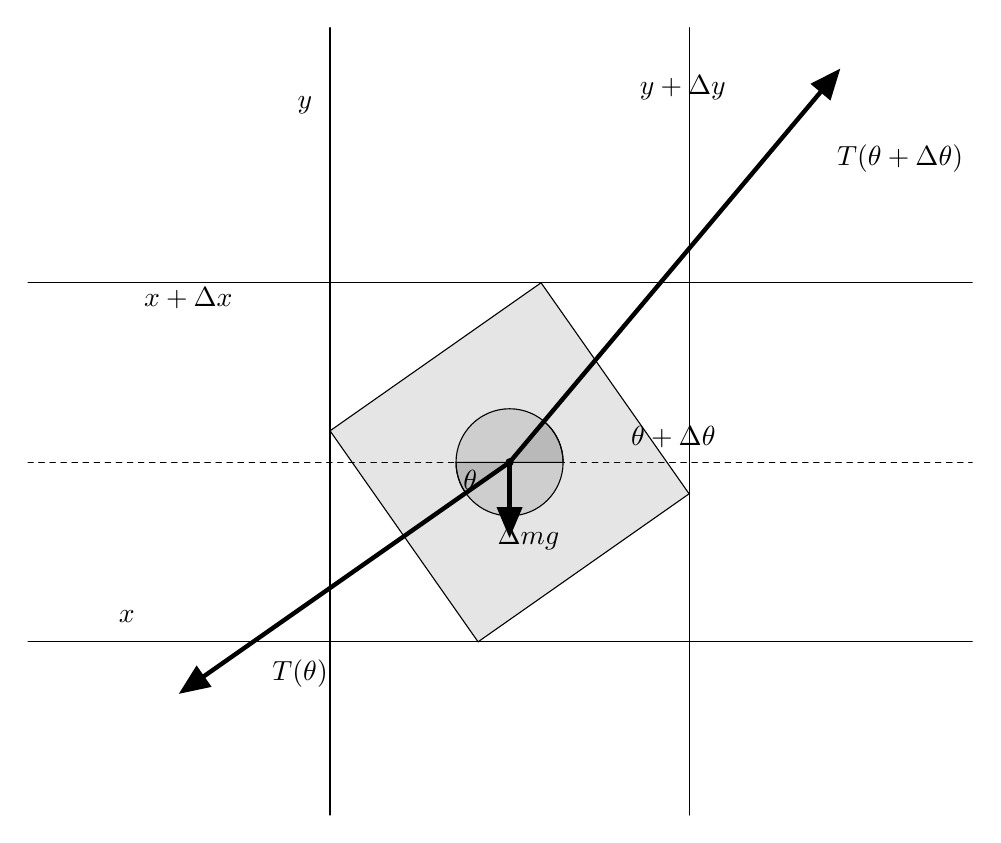
\begin{tikzpicture}[line cap=round,line join=round,>=triangle 45,x=2.0cm,y=2.0cm]
  \clip(-1,2) rectangle (5,7);
  \fill[fill=black,fill opacity=0.1] (1.86,3.1) -- (3.2,4.04) -- (2.26,5.38) -- (0.92,4.44) -- cycle;
  \draw [shift={(2.06,4.24)},fill=black,fill opacity=0.1] (0,0) -- (0:0.34) arc (0:215.05:0.34) -- cycle;
  \draw [shift={(2.06,4.24)},fill=black,fill opacity=0.1] (0,0) -- (-180:0.34) arc (-180:50.05:0.34) -- cycle;
  \draw (1.86,3.1)-- (3.2,4.04);
  \draw (3.2,4.04)-- (2.26,5.38);
  \draw (2.26,5.38)-- (0.92,4.44);
  \draw (0.92,4.44)-- (1.86,3.1);
  \draw [line width=0.4pt,domain=-1:5] plot(\x,{(-5.38-0*\x)/-1});
  \draw [line width=0.4pt,domain=-1:5] plot(\x,{(-3.1-0*\x)/-1});
  \draw [line width=0.4pt] (0.92,2) -- (0.92,7);
  \draw [line width=0.4pt] (3.2,2) -- (3.2,7);
  \draw [line width=0.4pt,dash pattern=on 2pt off 2pt,domain=-1:5] plot(\x,{(-4.24-0*\x)/-1});
  \draw [->,line width=1.6pt] (2.06,4.24) -- (-0.04,2.77);
  \draw [->,line width=1.6pt] (2.06,4.24) -- (4.16,6.74);
  \draw [->,line width=1.6pt] (2.06,4.24) -- (2.06,3.76);
  \fill [color=black] (2.06,4.24) circle (1.5pt);
  \draw[color=black] (0.02,5.28) node {$x+\Delta x$};
  \draw[color=black] (-0.37,3.26) node {$x$};
  \draw[color=black] (0.76,6.51) node {$y$};
  \draw[color=black] (3.16,6.62) node {$y+\Delta y$};
  \draw[color=black] (1.81,4.13) node {$\theta$};
  \draw[color=black] (3.1,4.4) node {$\theta+\Delta\theta$};
  \draw[color=black] (0.73,2.9) node {$T(\theta)$};
  \draw[color=black] (4.54,6.17) node {$T(\theta+\Delta\theta)$};
  \draw[color=black] (2.18,3.76) node {$\Delta m g$};
  \end{tikzpicture}
\end{center}

\begin{align*}
  \hat T: \qquad T(\theta)\cos\theta & = T(\theta + \Delta \theta)\cos(\theta + \Delta \theta) \\
  %\Delta m g & = T(\theta + \Delta \theta)\sin(\theta + \Delta \theta) - T(\theta)\sin\theta \\
  T(\theta) & = \frac{T(\theta + \Delta \theta)\cos(\theta + \Delta \theta)}{\cos\theta} \\
  T(\theta) - T(\theta + \Delta\theta)& = \frac{T(\theta + \Delta \theta)\cos(\theta + \Delta \theta)}{\cos\theta} - T(\theta + \Delta \theta) \\
    & = \frac{T(\theta + \Delta \theta)}{\cos\theta}(\cos(\theta + \Delta \theta) - \cos\theta) \\
  \\
  \lim_{\Delta\theta\rightarrow 0}\frac{T(\theta) - T(\theta + \Delta\theta)}{\Delta \theta} & = \lim_{\Delta\theta\rightarrow 0}\frac{T(\theta + \Delta \theta)}{\cos\theta}\cdot \frac{\cos(\theta + \Delta \theta) - \cos\theta}{\Delta\theta} \\
  -\frac{d}{d \theta}T(\theta) & = \frac{T(\theta)}{\cos\theta}\frac{d}{d\theta}\cos\theta \\
  \frac{d T}{d \theta} & = T(\theta)\tan\theta \\
  \ln\left(T(\theta)\right) & = C - \ln\left(\cos\theta\right) \\
  T(\theta) & = c \sec \theta
\end{align*}

\end{document}
